\documentclass[10pt,a4paper]{article}

\usepackage[top=1.5cm, bottom=1.5cm, left=1.6cm, right=1.6cm]{geometry}
\usepackage{graphicx}
\usepackage{subcaption}
\usepackage{booktabs}
\usepackage{amsmath}
\usepackage{microtype}
\usepackage{parskip}
\usepackage{caption}
\usepackage{float}

\graphicspath{{figures/}}
\captionsetup{font=footnotesize, labelfont=bf}
\setlength{\parskip}{0.1em}
\linespread{0.95}
\usepackage{titlesec}
\titlespacing*{\section}{0pt}{0.5em}{0.18em}
\titleformat{\section}{\normalfont\large\bfseries}{\thesection}{0.6em}{}
\setcounter{topnumber}{3}
\renewcommand{\topfraction}{0.92}
\renewcommand{\textfraction}{0.05}
\renewcommand{\floatpagefraction}{0.85}

\title{\vspace{-1.2em}Is Chain of Thought an Interchangeable Scratchpad?\\
\large J-space ablation versus external reasoning across problem difficulty (Qwen3-4B)}
\author{Shivam Singhal, Harvard CS 2881, Homework Zero}
\date{5 August 2026}

\begin{document}
\maketitle
\vspace{-3.3em}
\small

\section{Hypothesis}
In the paper, the authors ablate the ten most active directions in the J-space at every
token position across a band of middle layers, and find that GSM8K solved with a chain of
thought (CoT) survives this ablation while the same problems answered directly do not.
They conclude that the page and the J-space workspace are partially ``interchangeable
scratchpads.'' To interrogate this, we ask two questions. First, and as our main
investigation, what is the relationship between the internal and external scratchpads?
Second, how much protection does the CoT provide as problems harden?

For the first question, the authors suggest that CoT survives because the model
``externalises'' onto the page, yet they do not investigate what this externalisation
means. We consider four mechanism hypotheses.
\begin{enumerate}\setlength\itemsep{0.1em}
\item \textbf{(exchange)} externalisation actually \emph{removes} the representation from
the J-space, which is no longer needed to hold it.
\item \textbf{(duplication)} externalisation merely \emph{duplicates} information that
continues to be held in the J-space.
\item \textbf{(complementary)} the externalised and internal contents are complementary,
a division of labour.
\item \textbf{(epiphenomenal)} the correlation is unrelated to storage altogether. Every
generated token buys another forward pass, so the benefit could be extra serial
computation rather than anything written down.
\end{enumerate}

For the second question, we hypothesise \textbf{(H1)} that the protection offered by CoT
is roughly constant across difficulty. This seems intuitive from the original paper as a
genuinely interchangeable scratchpad that substitutes for the damaged workspace on
grade-school problems should do the same on harder ones. We note in advance that the cross-dataset
comparison can only weakly test this, since GSM8K, MATH-500 and AIME differ in topic, format
and contamination as well as difficulty.  We hypothesise our results will show the
following, GSM8K at $\sim$90\% with CoT and $\sim$25\% direct with AIME direct at
floor, a guess that the model can chain three to seven operations internally without a
page (the serial budget $D$ of \S2) with behavioural collapse within $\pm2$, and a
floor rule, a dataset with zero
clean direct accuracy cannot inform the comparison.

\section{Experiment design}
We first validate the pipeline by reproducing the original paper's Figure-24 contrast, crossing
\{CoT, direct\} with \{clean, light, medium, heavy ablation\} on GSM8K. The reproduction succeeds
(Fig.~\ref{fig:rep}), with CoT essentially unaffected at any strength.

To test our 4 mechanistic hypotheses, we measure \emph{occupancy}, how strongly the model
is internally representing a token $v$ at a given layer and position, the projection
$\mathrm{occ}(v,\ell,t)=\langle h_{\ell,t},\hat{\jmath}_v\rangle$ onto $v$'s J-lens
direction.

We investigate hypotheses (1, exchange) and (2, duplication) with a \emph{maintenance
test} of whether the model holds a value internally across a gap. The model reads a
definition such as $x=7$, then a stretch of unrelated text, then a question asking for
the value. Occupancy alone is not decisive here, because the definition stays
visible and the model can always re-read it rather than hold it, so we make re-reading impossible. An attention mask hides the definition from
the question onward while the gap stays readable, so re-reading is blocked but carrying
the value through the gap positions is not. A severed control masks the gap as well,
so the value cannot get through at all, which sets the lower bound. A page condition
keeps the mask but restates the value inside the gap, leaving a written copy readable,
as a CoT's page would be. A model holding the value internally loses nothing when the
definition is hidden. A model that answers by re-reading loses its only source and
falls to the severed floor.  We test hypothesis (1) a second way with a \emph{dual-task probe}. The model
holds an unrelated single-token word while solving, and we measure recall of the
word afterwards and its occupancy during solving. If writing frees capacity, both
should presumably be stronger with CoT than without. Next, a \emph{correspondence test}
allows us to investigate hypothesis (3, complementary). If the division of labour were
by content kind, the workspace would hold content of a different kind from what a CoT
writes, so it should not represent page-type values. We measure occupancy of the intermediate values of
small arithmetic chains in two settings, answered directly, where nothing is
externalised, and answered with the model's own chain of thought, the scenario the
hypothesis is actually about, where we read each value's occupancy as the model writes
it, during the later lines, and at the line that uses it. If the values appear in the
workspace, it handles page-type content and the by-content reading fails. We investigate hypothesis (4, epiphenomenal) with a \emph{prefix-rescue test}. We prefill an ablated
model with its own correct reasoning, with content-free filler of identical token length,
or with another problem's reasoning. If filler rescues as well as content, the benefit
might be better compute in chain of thought, not externalisation of representations.
Finally, to characterise the capacity CoT putatively replaces, a
\emph{depth ladder} of sequential single-digit chains (lengths 2--8, each line consuming
the previous value) is answered without CoT, measuring accuracy and the serial budget
$D$, the largest length whose answer still surfaces in the readout before emission.

For the second question, we repeated the validation experiment on MATH-500, stratified
over its five levels, and both AIME exams.

\begin{figure}[t]
  \centering
  \begin{minipage}[t]{0.37\linewidth}
    \centering
    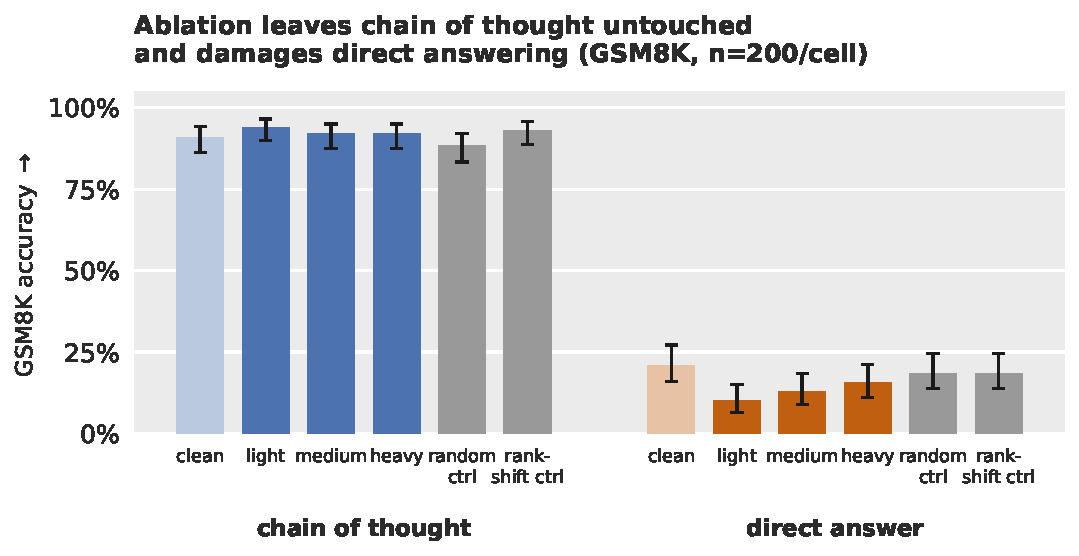
\includegraphics[width=\linewidth]{fig_gsm8k_retention}
    \captionof{figure}{Reproducing the paper's Figure-24 contrast on Qwen3-4B (error bars
    are Wilson 95\% CIs, $n{=}200$ per cell). Ablation at any band width leaves chain of
    thought untouched while damaging direct answering, and the norm-matched random
    control shows the damage requires the selected directions.}
    \label{fig:rep}
  \end{minipage}\hfill
  \begin{minipage}[t]{0.58\linewidth}
    \centering\footnotesize
    \setlength\tabcolsep{2pt}
    \begin{tabular}{lrrrrrrl}
    \toprule
     & \multicolumn{2}{c}{clean} & \multicolumn{2}{c}{medium abl.} & \multicolumn{2}{c}{retention} & \\
    dataset & CoT & direct & CoT & direct & CoT & direct & $\rho$ [95\% CI] \\
    \midrule
    GSM8K ($n{=}200$)    & 91.0\% & 21.0\% & 92.0\% & 13.0\% & 1.01 & 0.62 & 1.63 [1.05, 2.73] \\
    MATH-500 ($n{=}243$) & 65.0\% & 23.9\% & 67.9\% & 19.8\% & 1.04 & 0.83 & 1.26 [0.88, 1.84] \\
    AIME ($n{=}60$)      & 23.3\% & 0.0\%  & 18.3\% & 3.3\%  & 0.79 & --   & undef.\ (floor) \\
    \bottomrule
    \end{tabular}
    \captionof{table}{The difficulty axis. Retention is ablated accuracy over clean
    accuracy within one mode, so 1.0 means ablation cost nothing. AIME's $\rho$ is
undefined by the floor rule (clean direct $0/60$). CoT cells on MATH-500 and AIME are budget-limited floors (124--135/243
    and 59/60 truncated).}
    \label{tab:difficulty}
  \end{minipage}
\end{figure}

For controls, we considered that our ablations could reflect any sufficiently large
perturbation rather than the J-space specifically. A \emph{norm-matched random control}
removes an equal-norm component in random directions. A \emph{rank-shifted control} removes lens ranks 51--60 instead of the true
ablation's ranks 1--10. If damage came from removing lens
directions as such rather than the most active ones, it would hurt as much. The paper's method also includes an exclusion filter, which never ablates a direction
whose token the clean model already ranks in its top ten next-token predictions. In
direct answering the very next token \emph{is} the final answer, so this filter can
shield the answer itself from ablation and distort the CoT-direct comparison, so we
made it toggleable and checked the contrast without it.

\section{Experimental details}
We quantify damage with two ratios. \emph{Retention} is ablated accuracy divided by
clean accuracy within one answering mode, so a retention of 1.0 means the ablation cost
nothing. The \emph{protection ratio}
$\rho=\mathrm{ret}(\text{CoT})/\mathrm{ret}(\text{direct})$ then compares the two modes,
and is left undefined wherever clean direct accuracy sits at the floor.

The reference implementation provides lens fitting and readout only, so the intervention
itself is ours. At every position we score the vocabulary as
$W_U(\mathrm{norm}(J_\ell h))$, select the ten most active directions, and remove their
span from the residual by least squares, with a paired clean forward pass supplying the
exclusion filter. Our generation loop matches HuggingFace \texttt{generate()} token for
token with ablation off, and our occupancy measure reproduces the reference readout's
ordering (Spearman $\geq0.994$). We use the public
pre-fitted Qwen3-4B Jacobian lens, and place the paper's bands by depth fraction at
layers 22--26, 19--28 and 15--32 of 36. Unless stated otherwise, each cell contains
$n{=}200$ problems (MATH-500 $n{=}243$,
stratified, and AIME its full 60 problems) with one sample per
problem at $T{=}0.6$ and seed 0. Answers are extracted from the generated text, with
\texttt{math-verify} handling MATH and AIME equivalence. Accuracies carry Wilson 95\%
intervals and ratios carry bootstrap intervals. Generation is capped at 2048--4096 new
tokens for CoT and 32 for direct answering, and exact dataset revisions are pinned in
the repository. Our main statistical weakness is sampling depth, one sample and one seed
outside the headline cells, which did replicate at a second seed (pooled $\rho=1.50$
[1.13, 2.03]). One tokenizer fact shaped every probe. Qwen3 tokenizes numbers digit by
digit, and multi-token values are exactly where the paper reports its readout degrading,
so every value we ask the lens to read is a single token. 

\section{Experimental results}
\textbf{Replication with controls (Fig.~\ref{fig:rep}, Table~\ref{tab:difficulty}).}
The paper's contrast reproduces cleanly. Chain of thought is untouched at every band
width (91.0\% [86.2, 94.2] clean against 94.0/92.0/92.0\% under light, medium and heavy
ablation), while direct answering falls from 21.0\% [15.9, 27.2] to 10.0--15.5\%, giving
$\rho=1.63$ [1.05, 2.73]. The controls then localise the damage. A norm-matched random
ablation and a rank-shifted ablation each retain 0.88 of clean performance where the
true ablation retains 0.62, so the harm is specific to the currently most active J-lens
directions rather than to perturbation as such. Removing the exclusion filter shifts
$\rho$ only from 1.63 to 1.57, so the mode contrast is not an artifact of the filter
either.

\textbf{Mechanism instruments (Fig.~\ref{fig:mech}).} In the maintenance test we found no internal holding. Once the definition is made
unreadable at the point of use,
accuracy collapses from 100\% to 13.5\% [8.1, 21.8], indistinguishable from the severed
lower bound of 12.5\% ($n{=}96$ per condition), while a restatement inside the gap
restores 100\%. The model does not carry even a
single literal digit across a thirty-token gap. It answers by re-reading, and gap occupancy is near zero. At least for literal
values at this scale, storage lives in the context, and with nothing held there is
nothing for the page to duplicate and nothing for writing to remove, so hypotheses (1)
and (2) both lose their premise.  The dual-task probe gave a consistent result. Recall of the held word stayed at ceiling in all four conditions ($\geq$117/120), but recall only
tests re-reading, since the word remains visible in the prompt, and the word's occupancy
showed no asymmetry between modes, so writing freed no measurable capacity. In the correspondence test, when the model solves a three-step chain directly, the intermediate values surface in the workspace in computation order
(Fig.~\ref{fig:mech}a), so the workspace represents the values a chain of thought
would write. The same holds when the model
reasons on its own page. While it writes a value in its own chain of
thought, that value is strongly present in the workspace ($z{=}1.20$, $n{=}69$), it
fades over the following lines (0.16) and returns where the value is used again (0.42,
Fig.~\ref{fig:mech}b). The by-content
reading therefore fails in both settings, and the storage picture from the maintenance
test reappears, values are touched while written or used and not kept in between.
Detectability of single digits is modest (AUC 0.67 [0.59, 0.74]
against our 0.70 bar). Finally, in the prefix-rescue test (Fig.~\ref{fig:mech}c), an ablated model handed
back its own correct reasoning recovers to 98.0\%, next to 99.3\% for its
clean counterpart, while filler of exactly the same length stays at the no-prefix
baseline (23.3\% against 19.3\%) and another problem's reasoning collapses to zero. What
the chain of thought contributes is therefore its content and not the forward passes its
tokens buy, and the epiphenomenal reading fails.

\textbf{The serial depth budget, or what the page replaces (Fig.~\ref{fig:ds}a).} With the depth ladder we investigate how many operations the model can chain
internally before it needs the page. The answer is two. Accuracy on the sequential chains is perfect at two
operations and collapses to 30\% at three ($n{=}30$ per length), and the fraction of
runs in which the answer surfaces in the readout before emission collapses at the same
length ($63\%\to30\%$). Our advance guess of $D\in[3,7]$ was therefore wrong, but the
predicted coincidence between the readout collapse and the behavioural cliff held
exactly.

\textbf{Difficulty (Table~\ref{tab:difficulty}).} On MATH-500 the pattern repeats,
with chain of thought losing nothing under ablation while direct answering is damaged,
and $\rho$ falls from 1.63 to 1.26 [0.88, 1.84]. On AIME the floor rule applies (clean
direct $0/60$), leaving CoT retention (0.79) as the only informative quantity. The
falling $\rho$ needs three qualifications before it can be read as weakening protection.
The cross-dataset difference is not individually significant ($\Delta\rho=0.40$
[$-0.45$, 1.42]). The fall at MATH-500 comes from the \emph{direct} arm recovering
(retention $0.62\to0.83$) rather than from CoT protection weakening ($1.01\to1.04$), so
any direct evidence of weakening rests on AIME alone. And the random controls on
MATH-500 ($\rho_{\text{rand}}=1.28$) and AIME are indistinguishable from the true
ablation, so direction-specific protection is established only on GSM8K (random $\rho$
1.10 against 1.63). On the axis that actually measures protection, CoT retention, the
data are consistent with H1.

\textbf{Scale (Fig.~\ref{fig:ds}b).} We applied one fixed recipe, the band at the same
depth fraction and each model read through its own lens, to three model sizes.
Direct-mode retention rises steadily with size (0.43/0.62/1.04 at 1.7B/4B/8B) while
chain of thought is never hurt. Taken literally the trend extrapolates to no damage at
all at Sonnet scale, which contradicts the paper's own result, and the contradiction dissolves
once we notice what is held fixed. The paper re-derived its band for each
model where we keep one recipe, and a fixed ten directions is a smaller share of a wider
residual stream. The panel therefore measures susceptibility to one recipe, not whether
a workspace exists at each scale.


\begin{figure}[t]
  \centering
  \begin{subfigure}[b]{0.275\linewidth}
    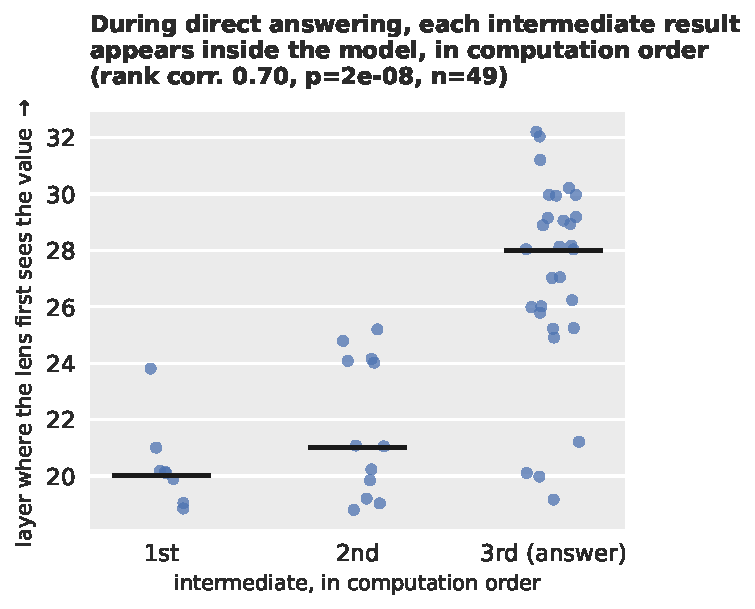
\includegraphics[width=\linewidth]{fig_numeric_ordering}
    \caption{}
  \end{subfigure}\hfill
  \begin{subfigure}[b]{0.275\linewidth}
    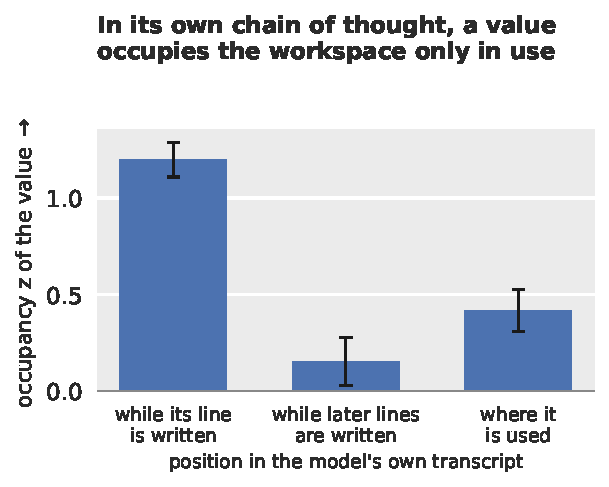
\includegraphics[width=\linewidth]{fig_cot_correspondence}
    \caption{}
  \end{subfigure}\hfill
  \begin{subfigure}[b]{0.305\linewidth}
    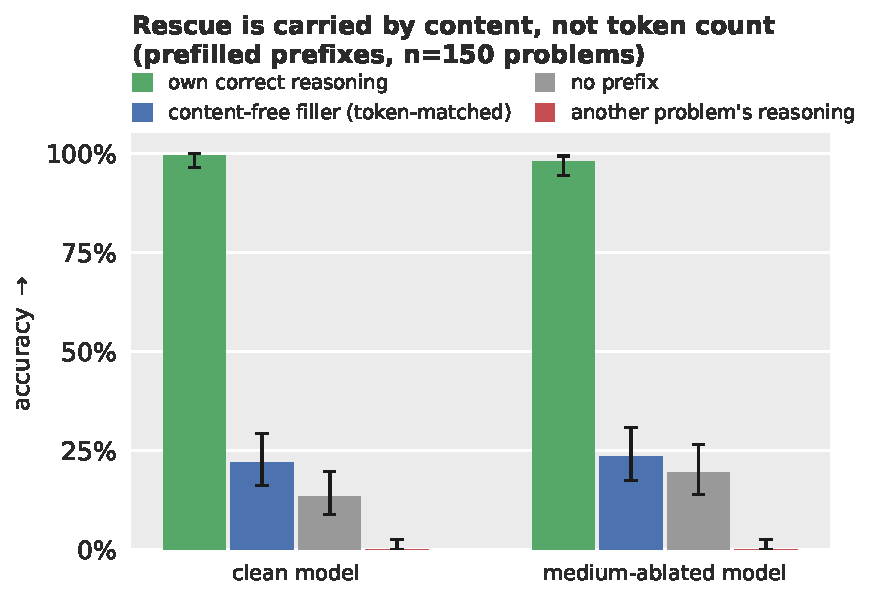
\includegraphics[width=\linewidth]{fig_prefix_rescue}
    \caption{}
  \end{subfigure}
  \caption{Mechanism results (error bars are Wilson 95\% CIs over problems). \textbf{(a)}
  The correspondence test. The model answers three-step arithmetic chains directly, and
  each dot marks one intermediate value, placed by its position in the computation (x)
  and the layer where it first becomes readable (y). Later values appear at later
  layers, so the workspace computes, in order, exactly the values a chain of thought
  would have written. \textbf{(b)} The CoT arm of the correspondence test.
  Mean occupancy of the first value inside the model's own chain of thought, in the
  three windows named on the axis (bars are 95\% CIs of the mean $z$). \textbf{(c)} The prefix-rescue test. Accuracy of the clean and
  medium-ablated models under each prefilled prefix. Only the model's own reasoning
  rescues the ablated model, filler of the same length does no better than no prefix,
  and each prefix acts the same without ablation.}
  \label{fig:mech}
\end{figure}

\begin{figure}[t]
  \centering
  \begin{subfigure}[b]{0.30\linewidth}
    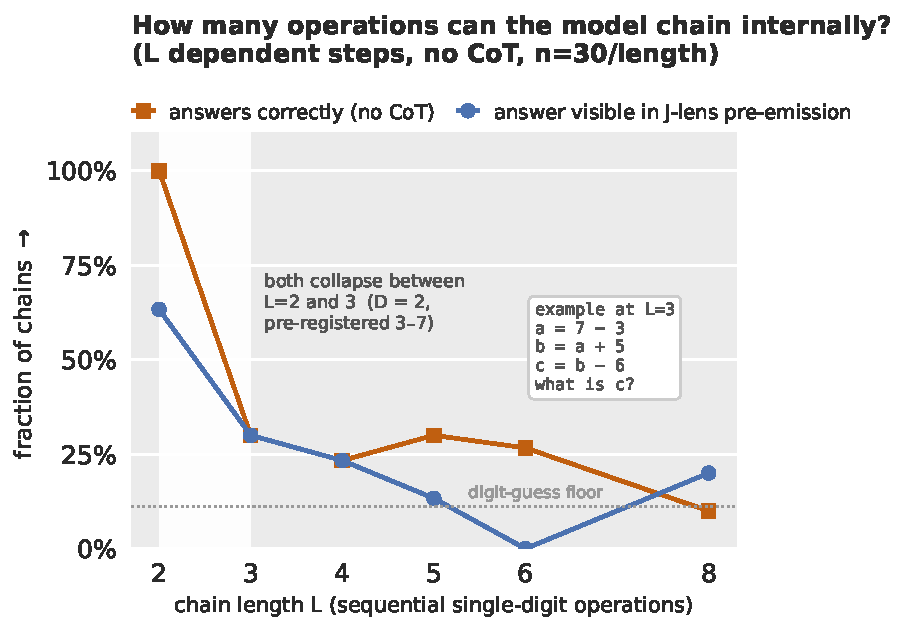
\includegraphics[width=\linewidth]{fig_depth_ladder}
    \caption{}
  \end{subfigure}\hfill
  \begin{subfigure}[b]{0.28\linewidth}
    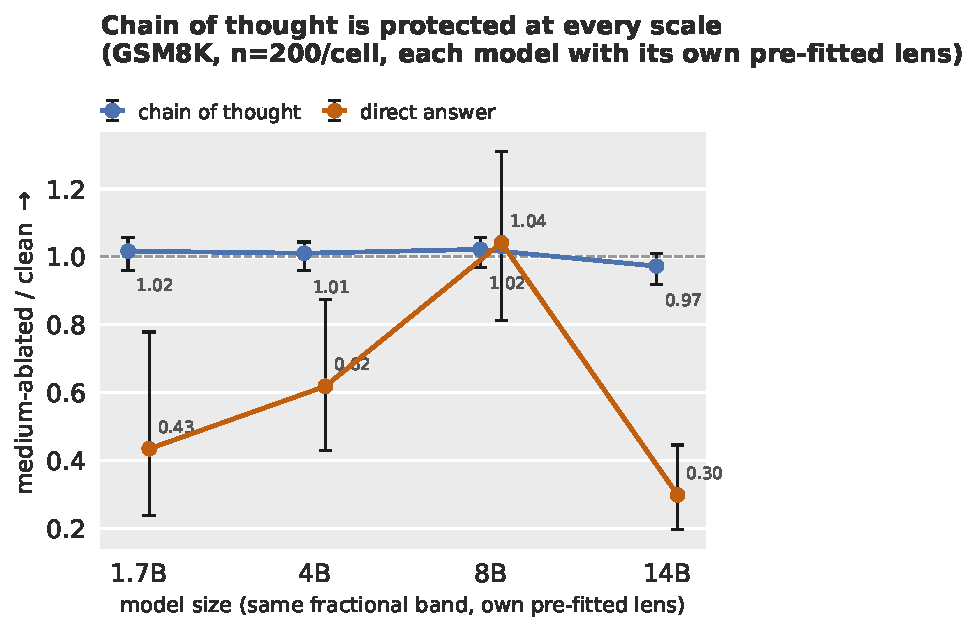
\includegraphics[width=\linewidth]{fig_scale_retention}
    \caption{}
  \end{subfigure}
  \caption{Capacity and scale (error bars are Wilson 95\% CIs over problems). \textbf{(a)}
  The depth ladder. Programs of $L$ chained single-digit operations (e.g.\ $a=7-3$, then $b=a+5$, then $c=b-6$) are answered without
  chain of thought.
  Accuracy and pre-emission surfacing of the answer collapse together between $L{=}2$
  and $3$, so the internal budget is two operations. \textbf{(b)} The scale sweep.
  Retention under medium ablation at three model sizes. Direct answering grows less
  susceptible with scale while chain of thought is never hurt.}
  \label{fig:ds}
\end{figure}

\section{Analysis of results}
We draw two conclusions, within the limits set out below. First, it is clear that a 4B model does possess a
selectively ablatable workspace, answering the original paper's open question about whether small
models had a J-space at all.
However, our epiphenomenalism and complementarity hypotheses were rejected outright, and we find that the J-space does not contain a duplicate of externalised representations in the chain-of-thought approach. Therefore, it is most likely that the externalisation of representations means that the internal space no longer contains those representations as prominently as before, though this longitudinal change is yet to be investigated.
Second, on difficulty,
chain-of-thought protection did not measurably weaken across more difficult datasets. CoT retention stayed at 1.01 and
1.04 on GSM8K and MATH-500, with only the uncontrolled AIME cell dipping (0.79),
consistent with H1, and the falling $\rho$ decomposes into direct-arm changes rather
than weakening protection.

Two limitations qualify these claims. Statistically, most cells carry one sample and one
seed, and the random controls are indistinguishable from the true ablation on MATH-500
and AIME, so direction-specific protection is established only on GSM8K. Mechanistically, the storage
probes used literal single-digit values read through a lens of modest sensitivity (AUC
0.67), and nothing in the maintenance gap gave the model a reason to carry the value,
so that result shows no default holding rather
than no capacity. All
evidence comes from one model, so confident general claims would need larger $n$, more
models, and adversarial probe variants. With more time we would pursue three directions. First, a properly powered version of
the difficulty comparison, with many seeds per cell and a per-item model across mode,
ablation and dataset, so any decline in protection is estimated rather than read off
two points. Second, a maintenance test of what the model can hold rather than what
it holds by default, warning the model that the definition will become unavailable and
asking it to remember the value, so success requires internal carrying. Third, whether the balance between internal and external
workspace shifts with the nature of the task, comparing problems that stress arithmetic, recall,
planning or verbal reasoning, and harder instances of each, asking when the model leans
hardest on the page.

\end{document}
